\documentclass{article}

\usepackage{tikz}

\begin{document}

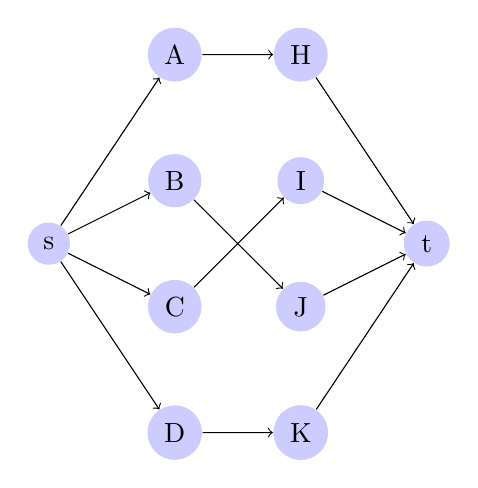
\begin{tikzpicture}
  [scale=.8,auto=left,every node/.style={circle,fill=blue!20},->]
  \node (G_S) at (0,5) {s};
  \node (G_1) at (2,8) {A};
  \node (G_2) at (2,6) {B};
  \node (G_3) at (2,4)  {C};
  \node (G_4) at (2,2) {D};
  \node (G_5) at (4,8)   {H};
  \node (G_6) at (4,6)  {I};
  \node (G_7) at (4,4)   {J};
  \node (G_8) at (4,2)  {K};
  \node (G_T) at (6,5) {t};
  \foreach \from/\to in {G_S/G_1,G_S/G_2,G_S/G_3,G_S/G_4,G_5/G_T,G_6/G_T,G_7/G_T,G_8/G_T,G_1/G_5,G_2/G_7,G_3/G_6,G_4/G_8}
    \draw (\from) -- (\to);

\end{tikzpicture}
\\
\\
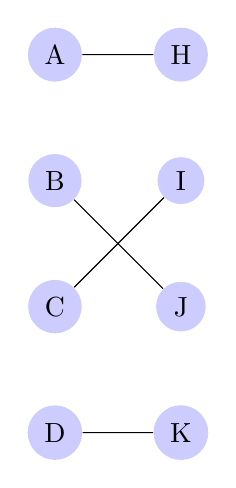
\begin{tikzpicture}
  [scale=.8,auto=left,every node/.style={circle,fill=blue!20}]
  \node (G_1) at (2,8) {A};
  \node (G_2) at (2,6) {B};
  \node (G_3) at (2,4)  {C};
  \node (G_4) at (2,2) {D};
  \node (G_5) at (4,8)   {H};
  \node (G_6) at (4,6)  {I};
  \node (G_7) at (4,4)   {J};
  \node (G_8) at (4,2)  {K};
  \foreach \from/\to in {G_1/G_5,G_2/G_7,G_3/G_6,G_4/G_8}
    \draw (\from) -- (\to);

\end{tikzpicture}

\end{document}